% !TEX program = xelatex
% !BIB program = bibtex
\documentclass%
	[type=bachelor,
	 printmode=auto,
	 bilinguallist = off,
	 seriftoc,
	]{cquthesis}%
\usepackage{cquthesis}
\usepackage{svg}
\usepackage{float}
\graphicspath{{images/}}

\begin{document}

\input{contents/cover}
\makecover %%% 封面部分


\frontmatter %%%前置部分(封面后绪论前)
%% 摘要
% \makeabstract
%% 目录,注意需要多次编译才能更新
% \tableofcontents
%% 插图索引,可选,如不用可注释掉
% \listoffigures
% \listoffiguresEN
% %% 表格索引,可选
% \listoftables
% \listoftablesEN
% %% 公式索引,可选
% \listofequations
% \listofequationsEN
% %% 符号对照表,可选
% \input{contents/denotation}

    \vspace*{\fill}\centerline{封二手动留白}\vspace*{\fill}
    \null\thispagestyle{empty}
    \addtocounter{page}{-1}
    \newpage

\mainmatter %%% 主体部分(绪论开始,结论为止)
%* 子文件的多少和内容由你决定(最好以章为单位),基本原则是提速预览、脉络清晰、管理容易。


% 
\chapter{绪论}

\section{机器学习的数学工具}
近年大火的机器学习和人工智能技术,均基于计算机的高计算性能实现,其内容主要包含对数据的处理、分类和预测,以及其对应的算法实现。

具体来说,机器学习\textbf{算法实现}的理论基础多为线性代数和概率论、统计论的相关知识,如回归分析、决策树、极值分析和最值分析、集成和聚类学习等。这些算法再经由计算机的软硬件算法,对处理过程加以优化,最终形成可调用的库供用户使用。例如,计算机的图形计算单元(GPU),其单指令多线程(以万为单位)的特性,决定了其适用于多维数据的快速计,并部署上述的各类算法。经优化,现在的GPU算力通常以GFLOPS(Giga-FLOPS, floating-point operations per second, 每秒10亿次的浮点运算数),实现了相较于CPU更快的发展,同时也促进了机器学习的革新进展。

所谓的\textbf{模型}一般用于解决特定性的问题,如YOLO用于机器视觉的多目标识别及分类,及BERT用于自然语言的语句识别及分类。当然,部分算法的代码实现,由于结合了多种算法思想,故也会被称作基本模型,例如概率图模型。前述模型则整合了多种基本模型,以应对复杂的现实问题。因此,非通用类的人工智能均由机器学习实现,本质仍是对数据的处理。\cite{周志华_2016, Sulmont_2019}

与之相对应,通用类的人工智能有机器学习(即数据处理)和生物神经模拟两类研究方向,但目前仍无突出优势和应用。

\section{人脸识别的社会应用}

人脸识别领域是机器学习视觉处理的重要组成部分,也是应用最广泛、社会争议最大的。虽然其名字中只有“识别”两个字,但其内容却包含了识别、分类甚至于特征替换等。经典的特征替换应用实例是DeepFake,这样一个模型可以将视频内的人脸进行替换,并在相当程度上让人类信以为真。虽然机器学习又可以通过该模型的训练规律,反向判断应用该模型“换脸”的视频,但只需稍微应用对抗学习的方法,机器便能自身演化形成独特的替换算法,而不被检测出规律性。\cite{Guera_2018}像这种引起社会恐慌的例子还有很多,在此就不一一列举。

不可否认的是,各类人脸识别系统在近几年如雨后春笋发展起来,但在真实场景的使用中,受限于硬件、成本等条件,这些系统使用的多半是传统的整体分类算法,其发展更多依靠的是数字处理能力的上升,以及智能终端的广泛普及,并已带来相当多的法理伦理问题。本次实验中,程序对数据集进行特征值提取处理后,再应用分类算法进行人脸识别的算法,也是一种简单的整体分类算法。以openCV库中人脸识别的类 \verb|FaceRecognizer| 为例,其包含Eigenface、Fisherface整体(代数特征)算法,以及LBPH局部特征提取算法。这些算法的不足和优化方向均是与脸部特征无关的图像特征,如人脸朝向、光照方向等。

商用级的人脸识别和应用还是以整体(Holistic)识别算法为主,并使用主成分分析(PCA)、独立成分分析(ICA)、线性判别分析(LDA)等作为识别不相关量,并进行降维的算法。在前沿研究和大数据处理方向,基于神经网络的人脸识别则经过卷积神经网络(CNN)等网络模型,被训练为提取偏好特征的特性(Feature)识别算法。基于神经网络的方案又被称为深度学习,它比传统机器学习需要更丰富多元的数据量,同时需要更多的计算性能,因此也更受人们的关注和争议。\cite{Zhao_2003, Anand_2017}

本次实验中要求以可交互界面(可视化用户界面,GUI)实现的特征脸(Eigenface)分类算法,使用的核心算法是主成分分析。实验成果参考了对应的算法,根据\autoref{cha:fr}详述的系统框架实现了相应的目标。具体的算法原理及性能、参数比较,将在\autoref{cha:bg}讨论。此外,为了对图像处理有基础的了解,本次实验还要求对图片进行色彩空间和空域滤波的预处理,具体结果将在\autoref{cha:re}讨论。









% \chapter{实验结果及分析、讨论}
\label{cha:re}

本章展示的实验数据,可通过调用程序相应部分复现。实验分析部分基于文献搜索结果。

\section{模块单元结果}

\subsection{图像的滤波处理}

对某相机拍摄的PNG图片,读取RGB颜色空间后,处理效果如\autoref{fig:hw1}:(其中从左上角,以先从左到右,再从上到下的顺序标数,第一张图像为原图,第二张图像为最大值取样,第三张图像为平均值取样,第四张图像为加权平均值取样(Luminance))

\begin{figure}[H]
    \centering
    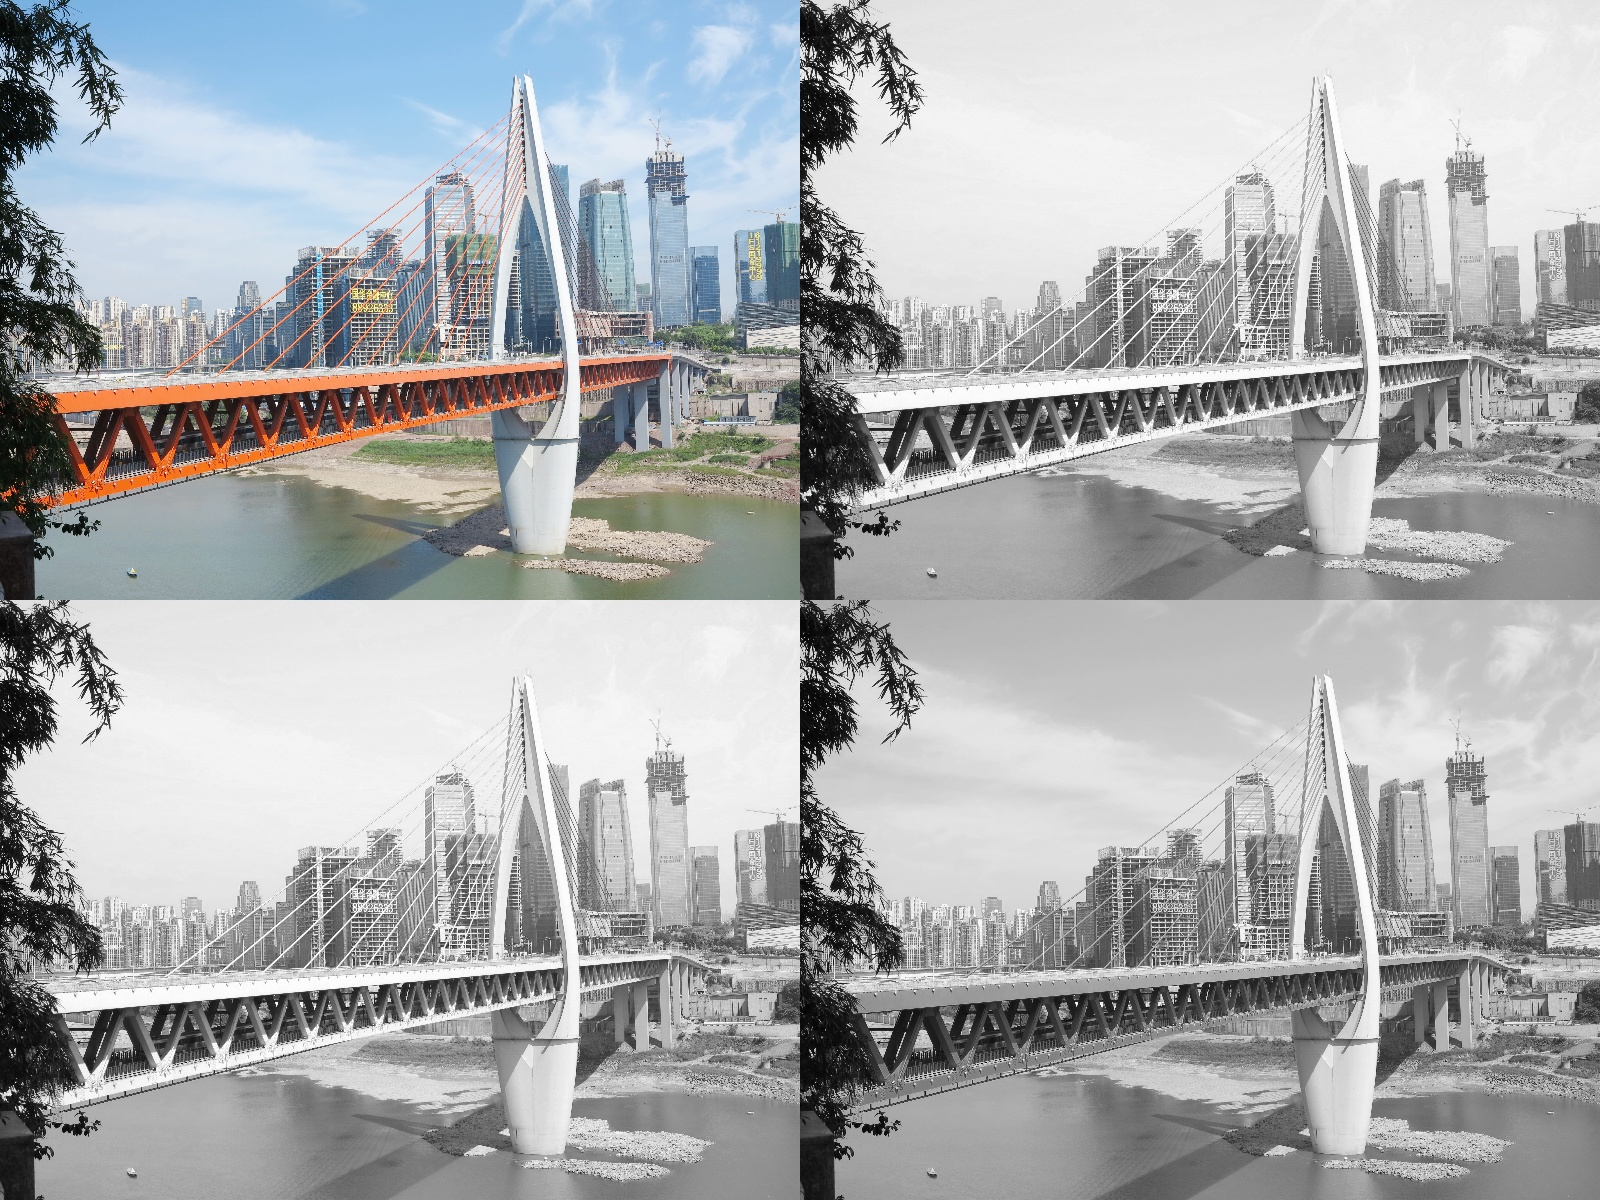
\includegraphics[width=.5\columnwidth]{hw1.jpg}
    \caption{灰度处理实验结果}
    \label{fig:hw1}
\end{figure}

根据人眼观察,在这种情况进行灰度空间转换时,使用加权平均值取样对这张图片的还原度最大,其明度较高的细节,如蓝天白云、红色桥梁等得到了充分保留。而后对数据库内人脸进行同等处理,也得到类似的直观结论。(所以电子行业用这个标准,还是有原因的!)

另外,在使用MATLAB或Python numpy库直接对读取图像进行处理时,很容易忽略数据类型的问题。对于正常的8位3通道图片,各像素点的数据均以\verb|uint8|的形式储存,在加权求和时,由于人脸数据库中图片明度普遍较高,故通道先求和,所得值将超过$2^8-1=255$,导致结果图像数据失真。可以调用平均值函数,或者数据类型转换来无损的解决这个问题。

需要注意的是,若要对这一结果进行深入研究,除了分析观察值外,还要结合其应用场景进行分析。此处,鉴于主流的图像处理工具(Matlab, OpenCV)均使用了Luminance加权平均值取样,故不再具体探讨其对实验结果的影响。为直击重点,本实验也不再探讨直方图优化、伽玛校正的原理,及其与灰度转换相结合的具体作用效果。

\begin{figure}[H]
    \centering
    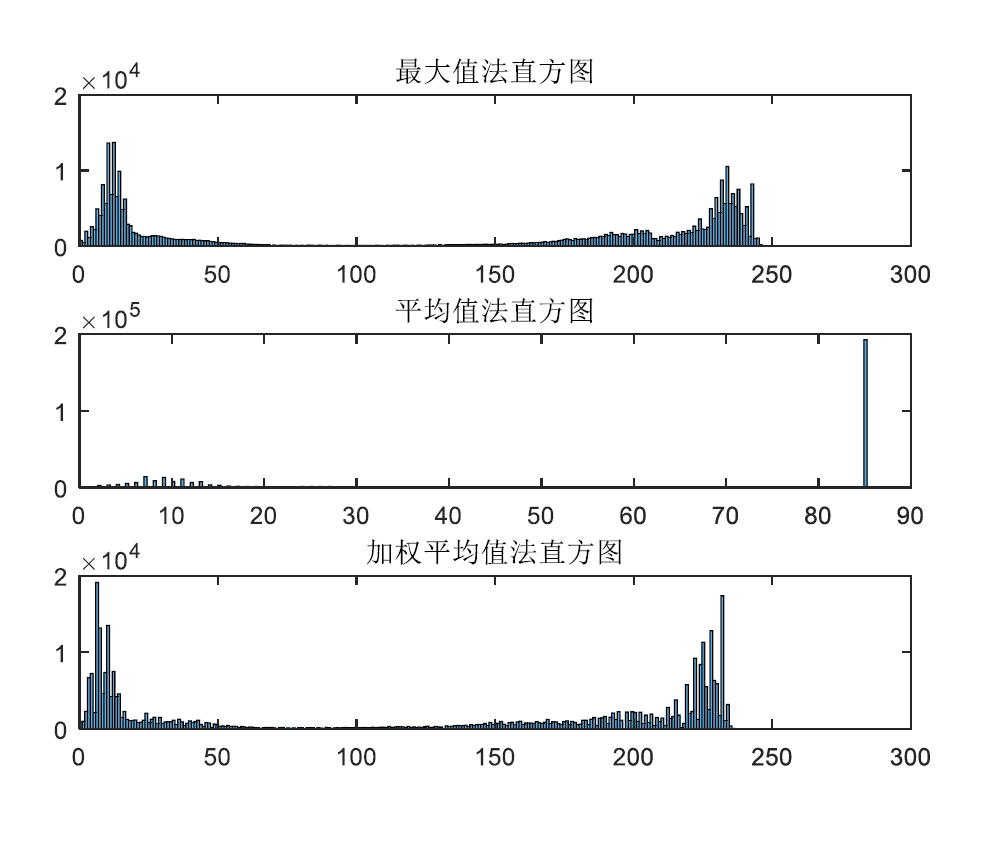
\includegraphics[width=.5\columnwidth]{hw1_add.png}
    \caption{某人脸图片经不同灰度处理后的直方图结果}
    \label{fig:hw1_add}
\end{figure}

\textbf{综上,经分析,程序主模块最终采用本部分的加权平均值取样部分(浮点输出)。}

\subsection{图像的主成分分析}

对数据库中训练库、测试库中的部分照片进行多种去噪处理,并将其图片输出,过中心的平行、垂直线上像素的R通道值的绘图数据,各像素点R通道8位值数据的直方图制作成图表,结果如下。

\begin{figure}[H]
    \centering
    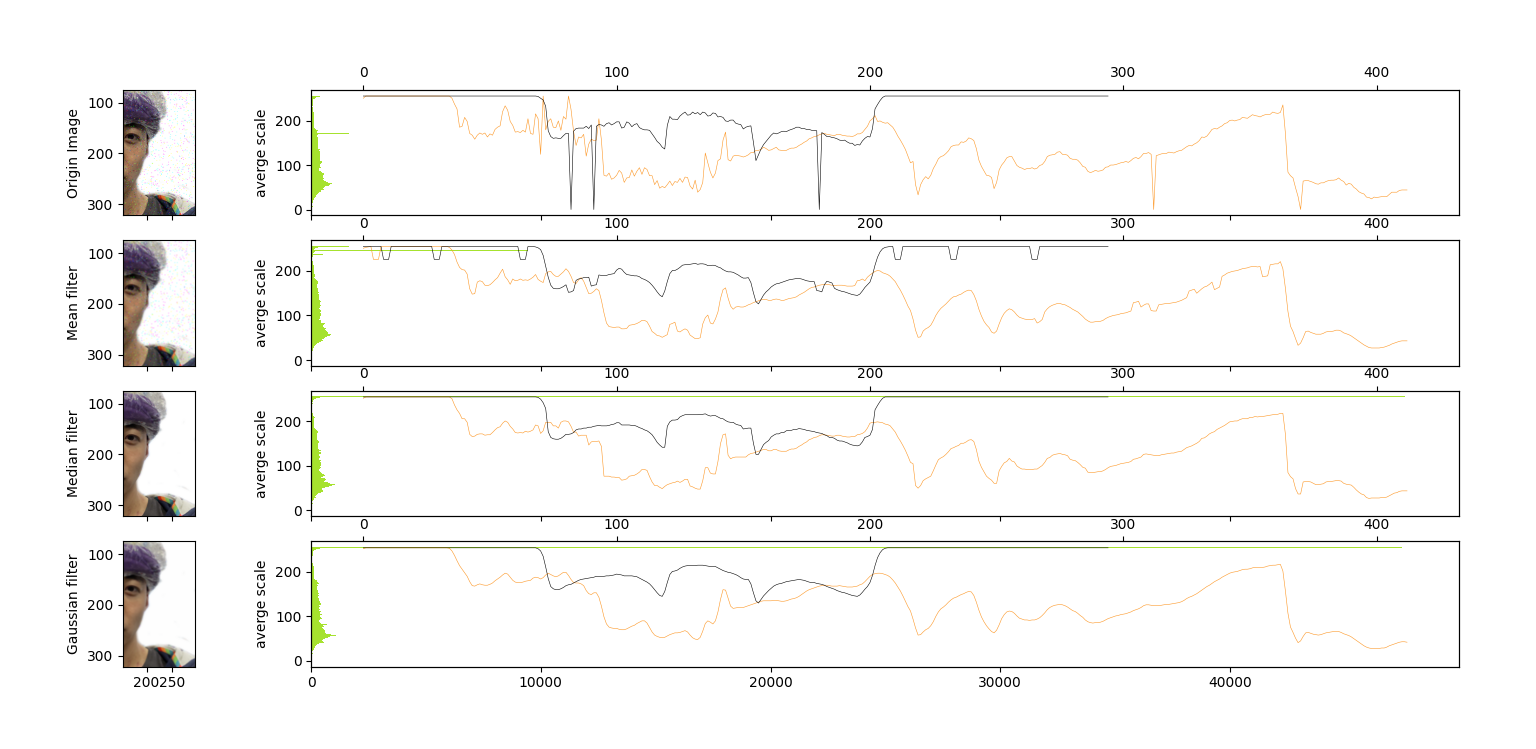
\includegraphics[width=.81\columnwidth]{hw2_fig1.png}
    \caption{三种滤波处理后的输出结果}
    \label{fig:hw2_1}
\end{figure}

\begin{figure}[H]
    \centering
    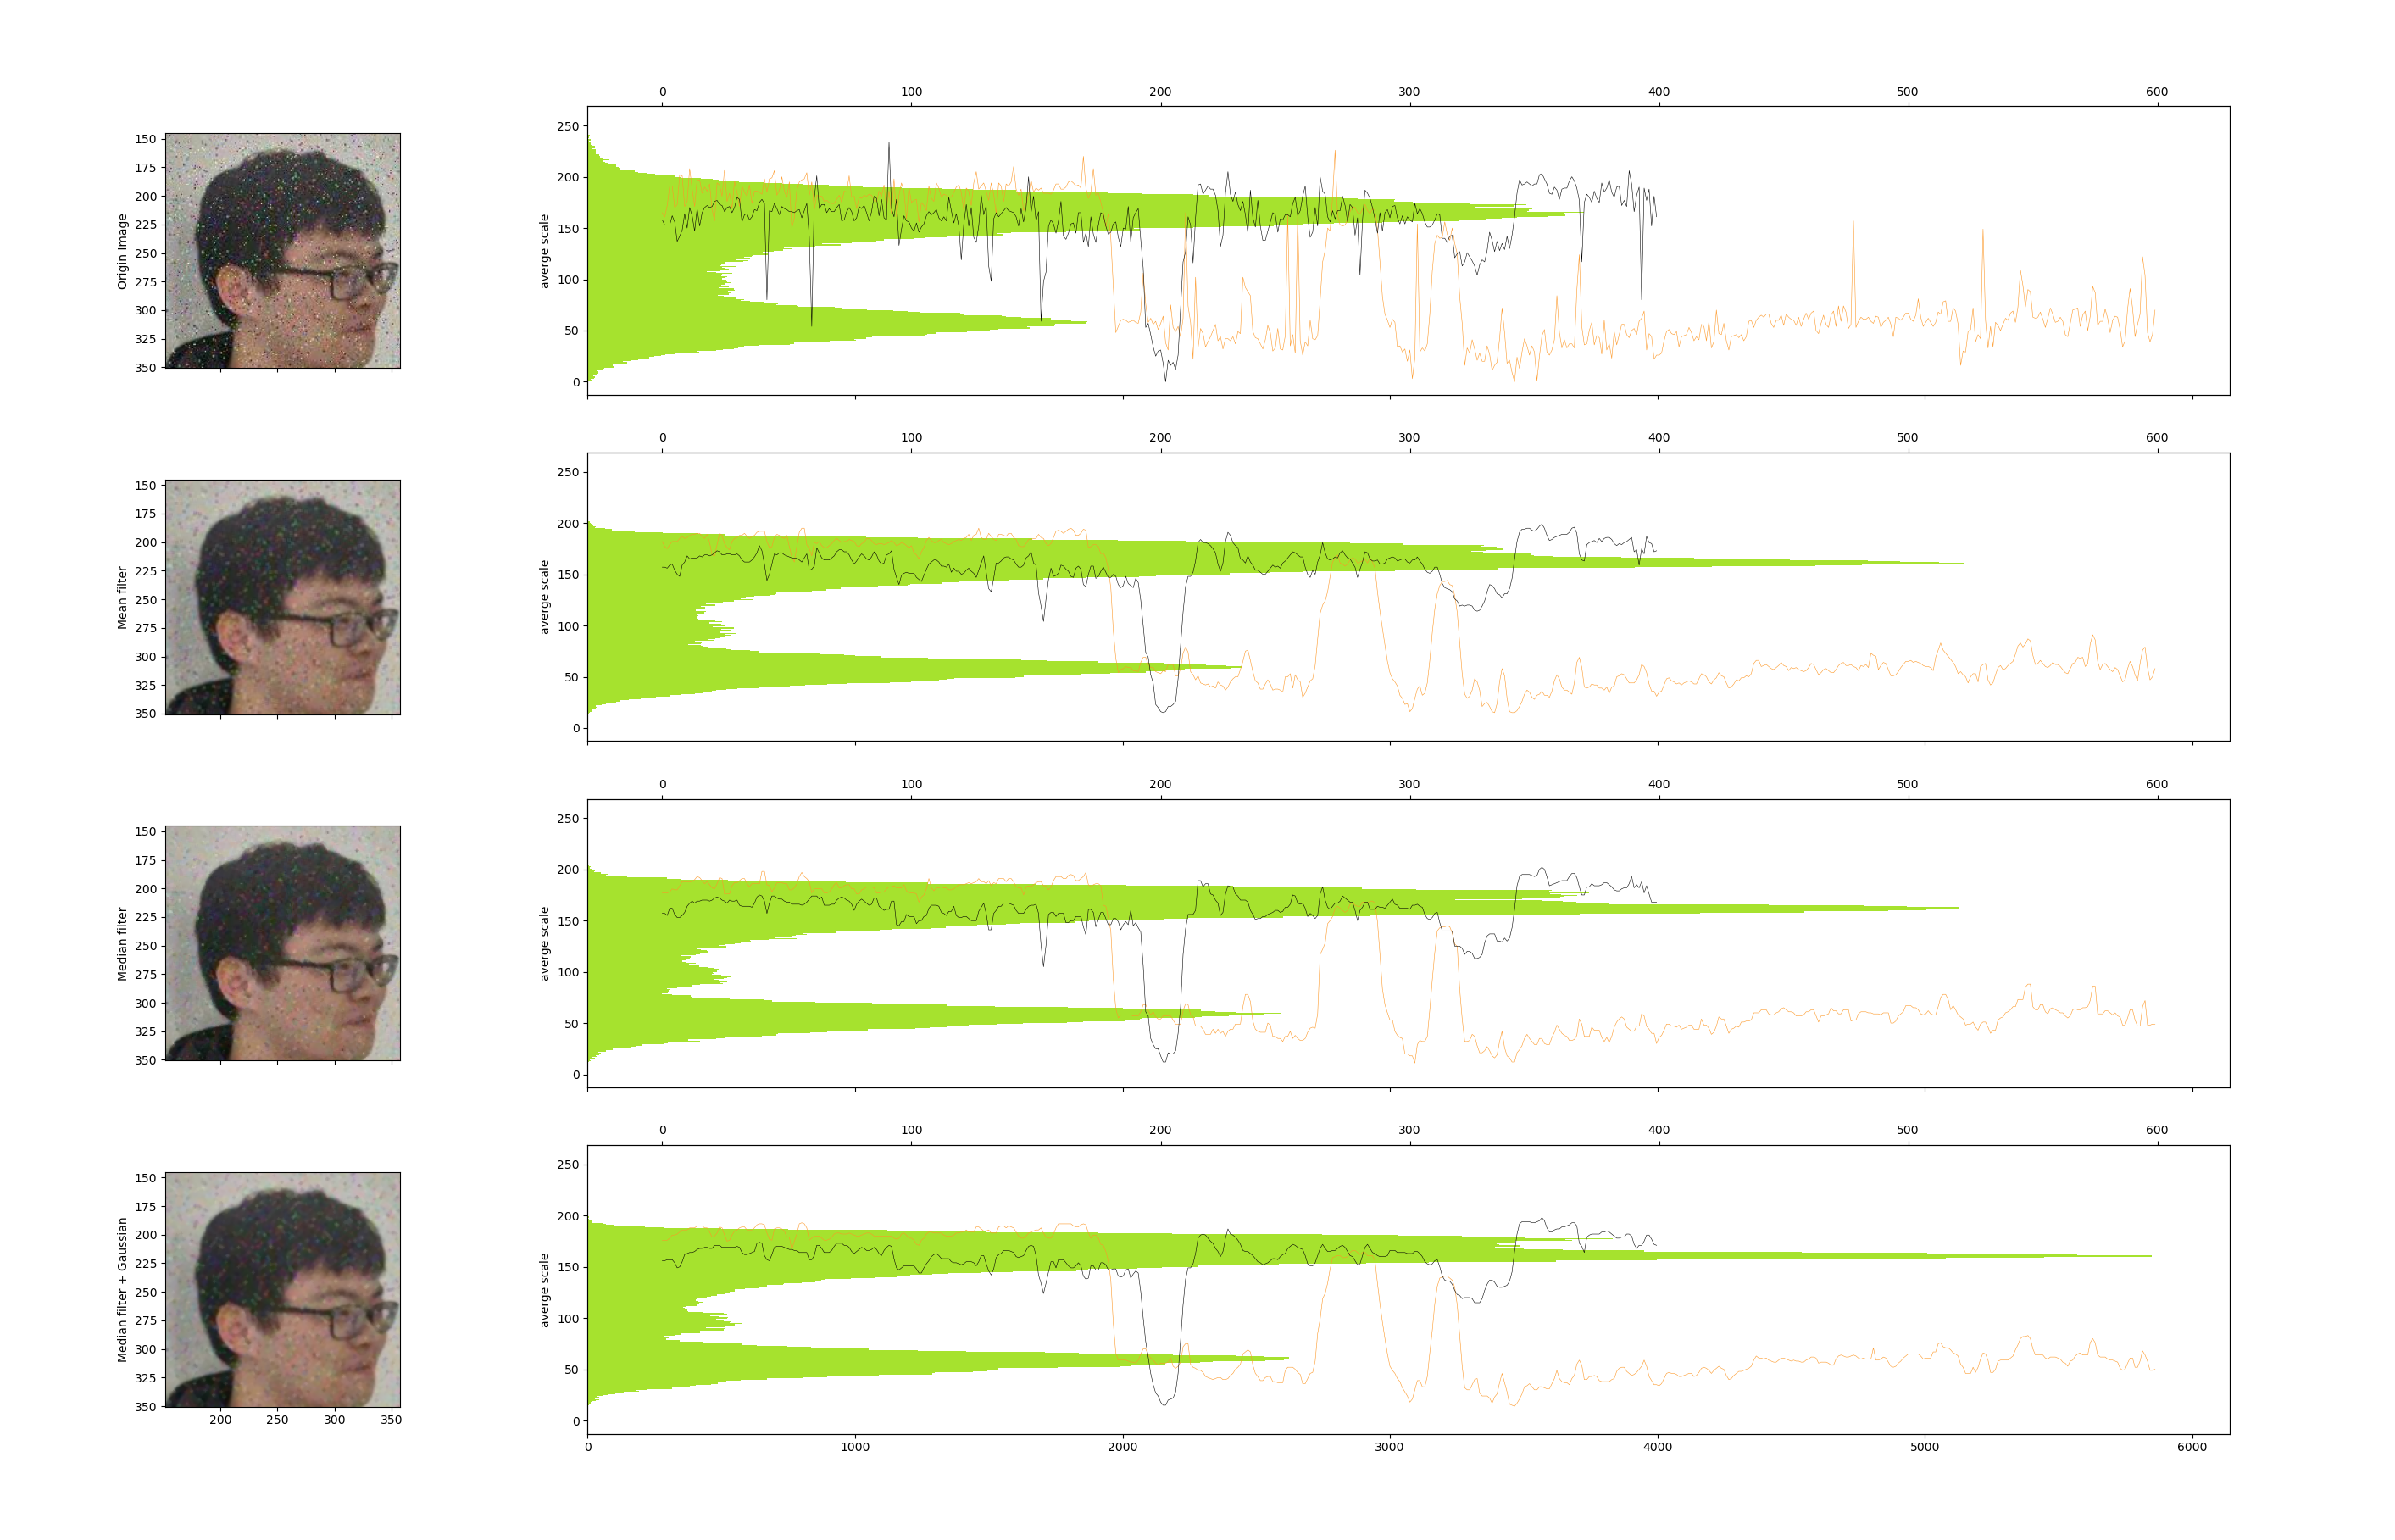
\includegraphics[width=.81\columnwidth]{hw2_fig2.png}
    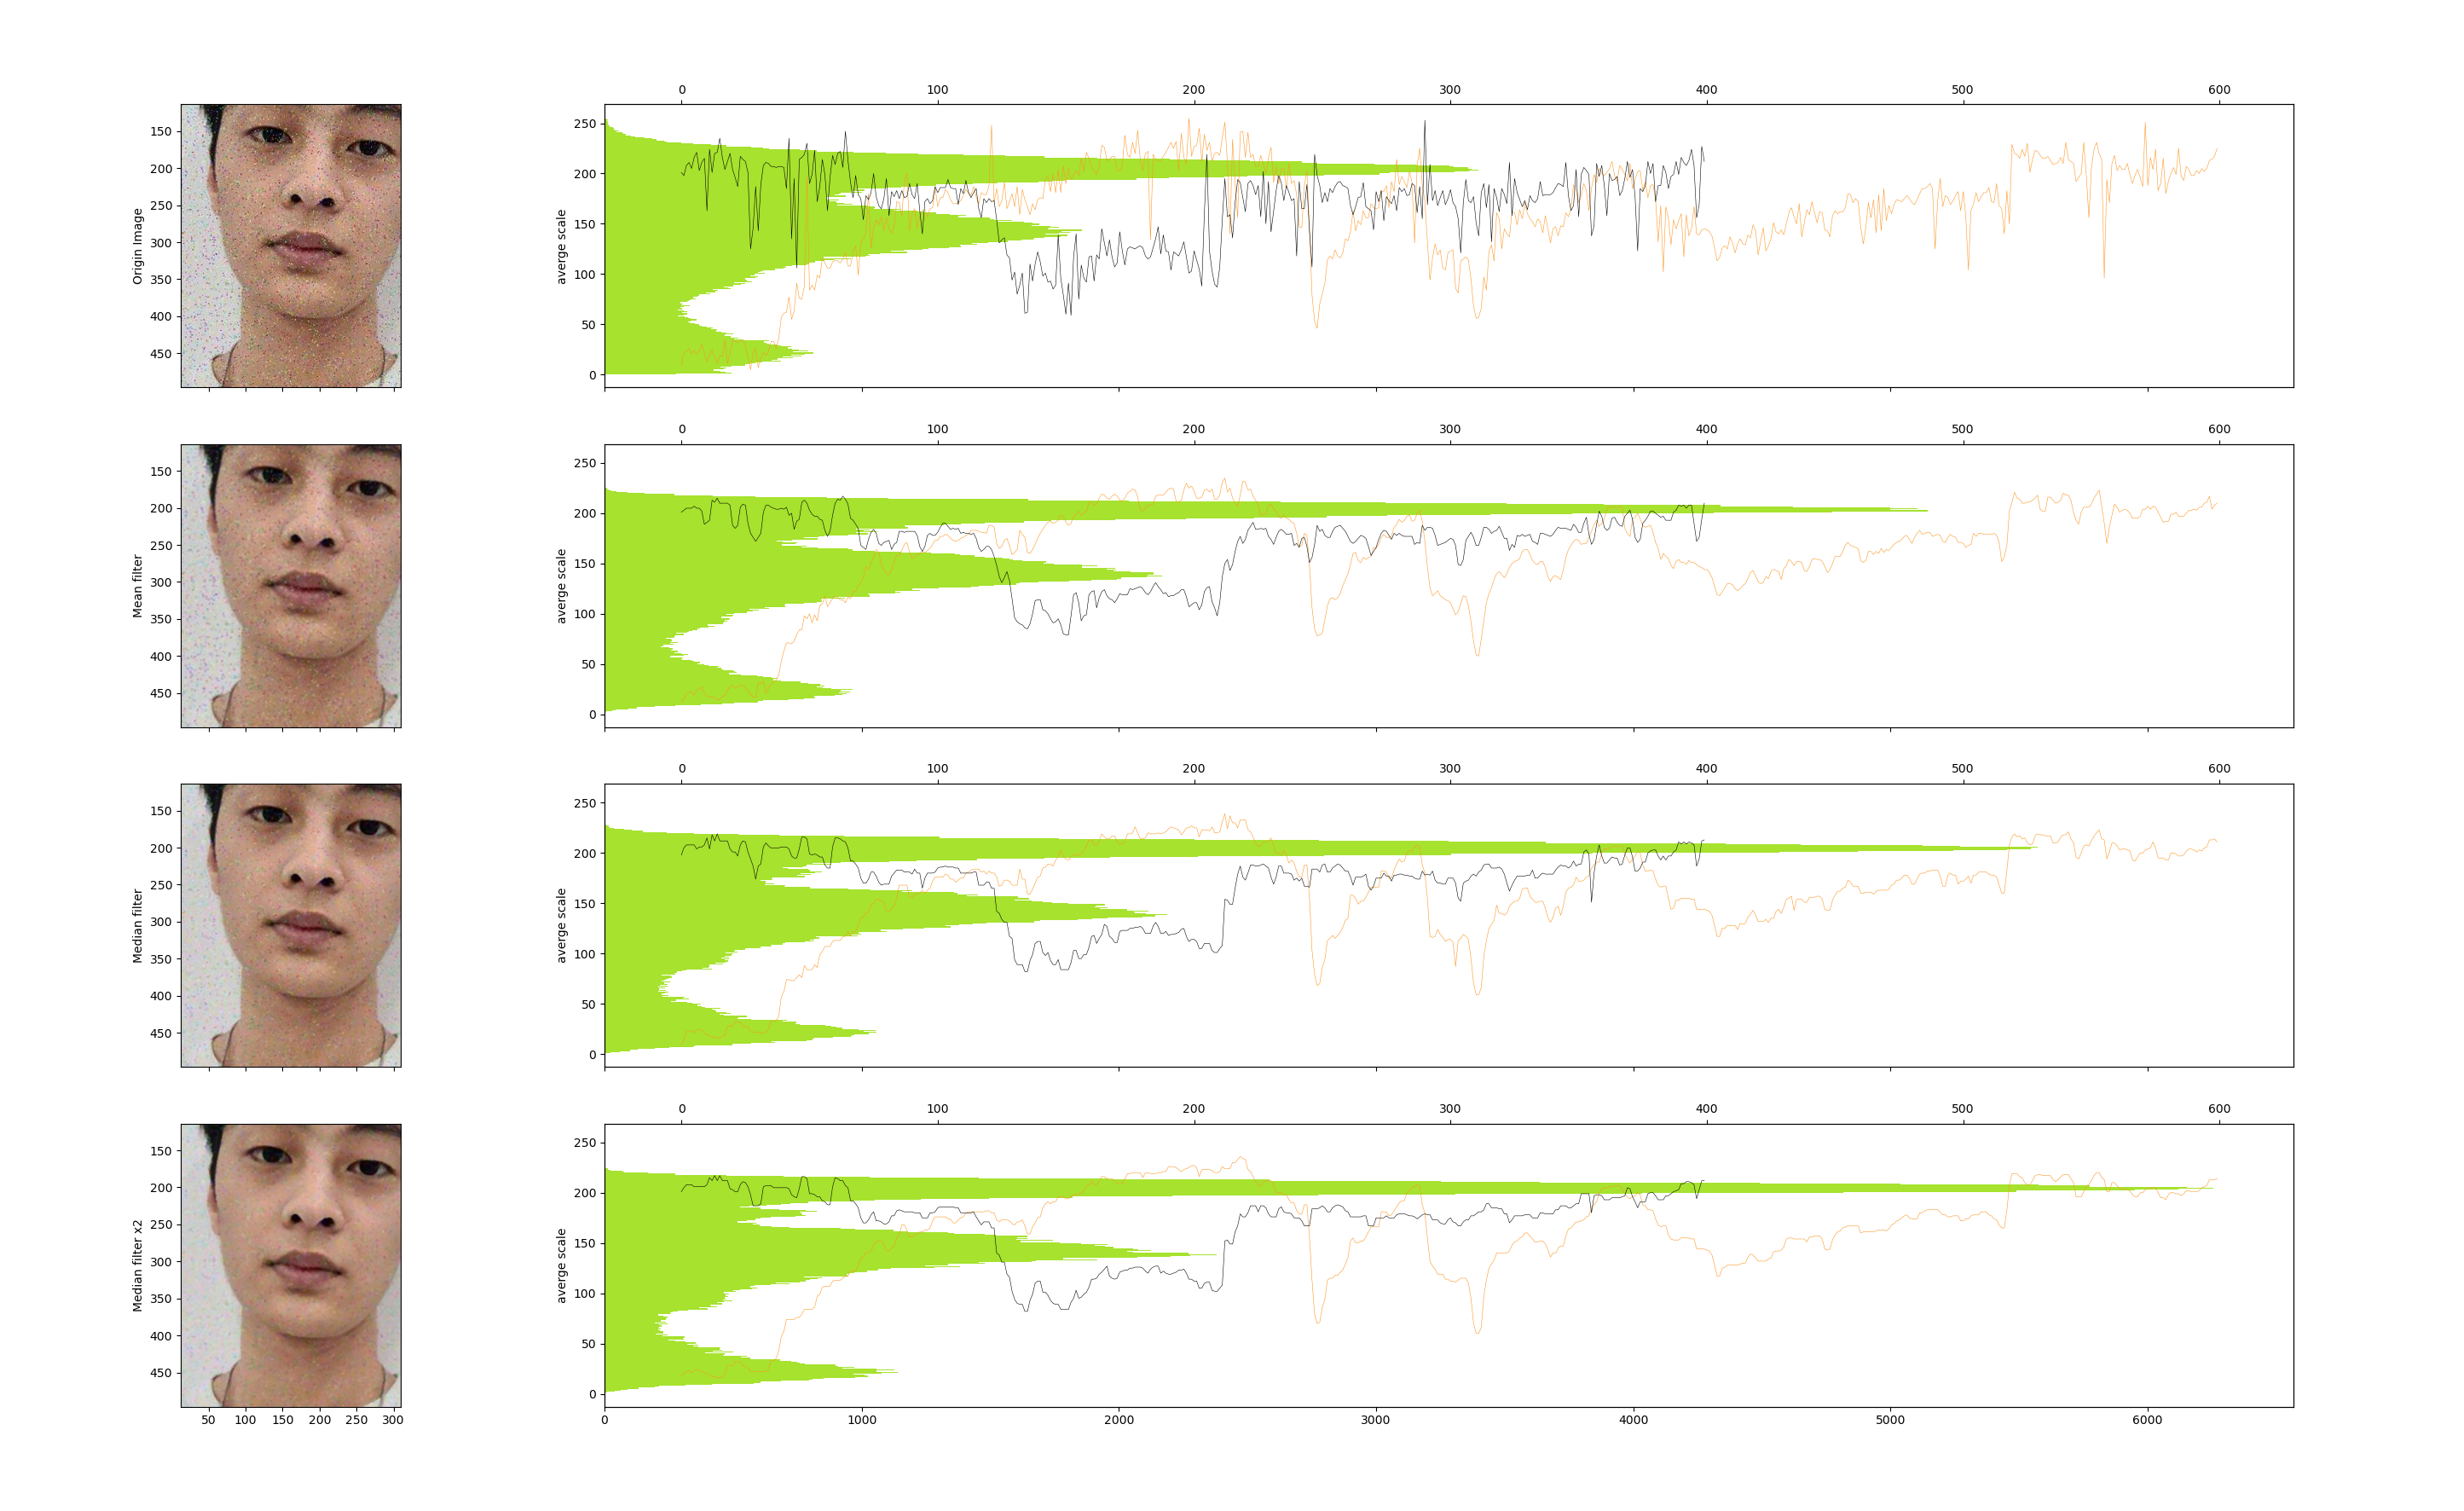
\includegraphics[width=.81\columnwidth]{hw2_fig3.png}
    \caption{分别展示了高斯滤波后中值滤波,两次中值滤波的输出结果}
    \label{fig:hw2_2}
\end{figure}

\autoref{fig:hw2_1}自上而下,展示了原图、均值滤波、中值滤波、高斯滤波的相应结果。可以发现均值滤波对椒盐噪声去除效果不好,另外两种滤波对简单的椒盐噪声去除效果较好。

\autoref{fig:hw2_2}的第一张后两行展示的分别是中值滤波、高斯滤波后中值滤波的输出结果,可以发现高斯滤波反而会增强高密度的椒盐噪声。其第二张后两行展示的分别是一次中值滤波、两次中值滤波的输出结果,可以发现二次中值滤波对噪声还有一定的削减作用。次数再次升高后,效果不再明显。

\textbf{综上,经分析,程序主模块最终采用本部分的中值滤波,并连续调用两次。}

\section{识别、交互系统结果}

\subsection{处理时间}
\label{sec:pca0}

\textbf{在本机}统计了训练模块中较为耗时的两部分:中值滤波处理和样本库主成分分析。不采用中值滤波的耗时为3.4\~4.9s,采用未加速的中值滤波耗时约为18min51s(每张图耗时约5s),numba加速的中值滤波耗时为15.5\~20.4s;主成分分析的耗时为4.2\~9.1s。

识别模块中耗时的主要部分为测试集批量读入,可同等看待。

\begin{figure}[h]
    \centering
    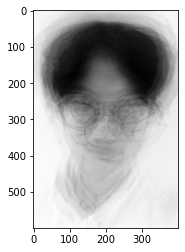
\includegraphics[width=.4\columnwidth]{eig_single.png}
    \caption{单组样本训练得到的第一个主特征,经可视化处理。}
    \label{fig:eig_single}
\end{figure}

\subsection{识别准确度}

对kNN分类算法和选取的主成分进行调整,发现当 $k=4$ 时,主成分最少仅需容纳前$12$维即可达到最佳识别正确率。仅\autoref{fig:class1}所示的样本无法被正确识别。增大主成分维数,识别结果基本不受影响。而增大 $k$ 值会导致部分测试样本匹配到其他类型的人脸。

样本12在$k$、$d$较高时才能被正常识别,如$k=27, d=185$。故样本12的训练集有过拟合的倾向。

\begin{figure}[H]
    \centering
    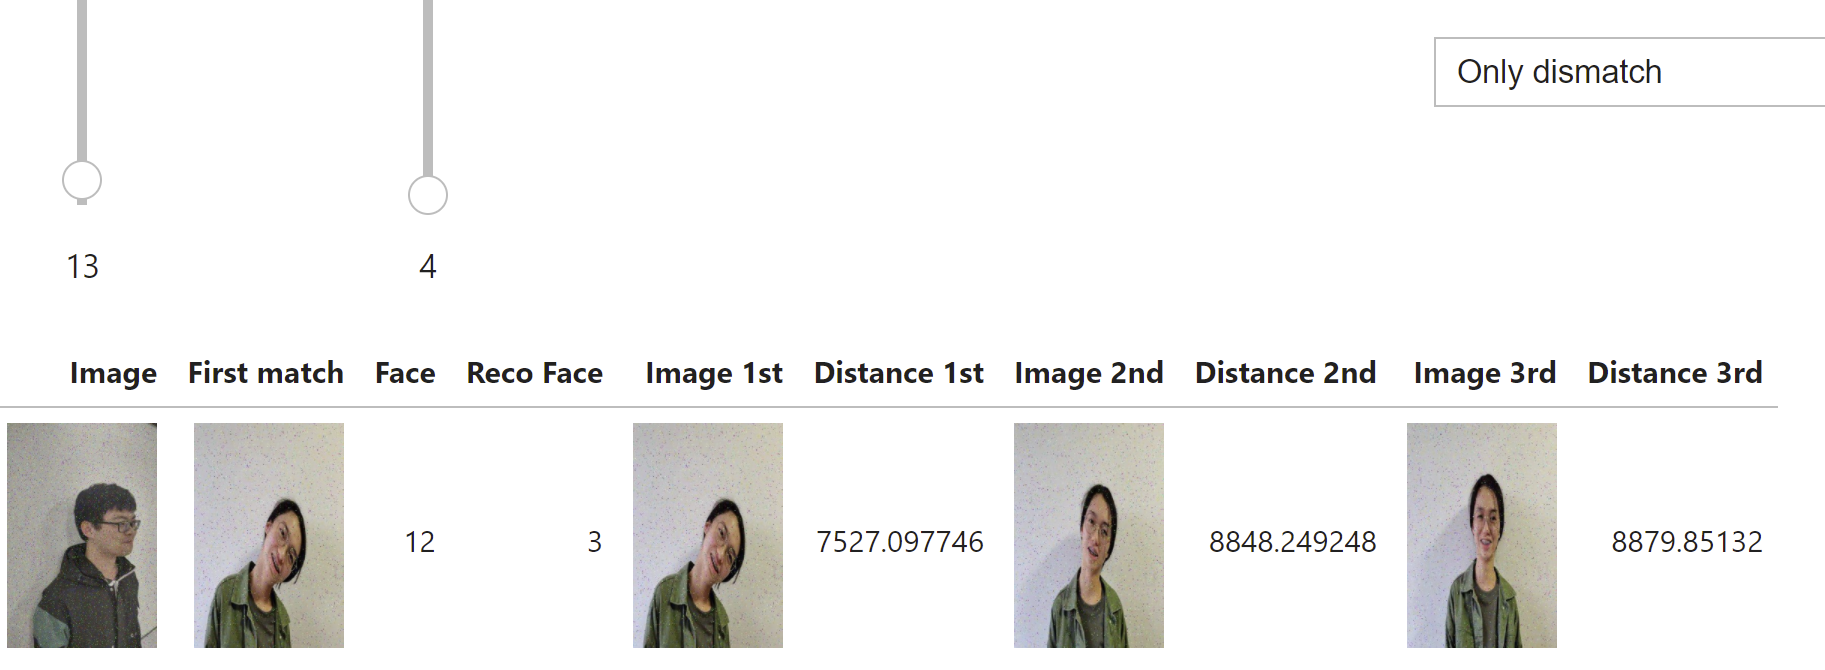
\includegraphics[width=.8\columnwidth]{class1.png}
    \caption{无法匹配的样本图片和识别输出结果}
    \label{fig:class1}
\end{figure}

\section{识别的调整及优化}

下列的数据展示了选取前$d$维主成分和$k$个临近数据集点后的分类情况。注意到有部分测试数据十分接近于训练数据,经查看文件,其中有部分测试图片与训练图片完全一样,另有一些是噪声不同。

\begin{minted}[breaklines]{xml}
d=20, k=4
test face 3 is too close to dataset(s3_1)?
test face 4 is too close to dataset(s4_3)?
test face 9 is too close to dataset(s9_1)?
12 3 [[9.92052951e+03 1.60000000e+01 3.00000000e+00]
 [9.92129420e+03 1.90000000e+01 3.00000000e+00]
 [1.06769758e+04 1.88000000e+02 2.40000000e+01]
 [1.06920015e+04 1.80000000e+01 3.00000000e+00]]
test face 22 is too close to dataset(s22_3)?
Error rate is 0.05.

d=120, k=4
test face 3 is too close to dataset(s3_1)?
7 15 [[[1.41684977e+04 5.80000000e+01 7.00000000e+00]
 [1.62357532e+04 1.23000000e+02 1.50000000e+01]
 [1.70395660e+04 1.20000000e+02 1.30000000e+01]
 [1.92705277e+04 1.22000000e+02 1.50000000e+01]]
test face 9 is too close to dataset(s9_1)?
12 3 [[1.61600607e+04 1.80000000e+01 3.00000000e+00]
 [1.71320333e+04 1.88000000e+02 2.40000000e+01]
 [1.71812421e+04 1.00000000e+01 1.00000000e+00]
 [1.78519738e+04 1.60000000e+01 3.00000000e+00]]
 test face 22 is too close to dataset(s22_3)?
Error rate is 0.1.
\end{minted}

那么我们拿完全不滤去噪声的训练集和测试集来跑跑看呢?好家伙,噪声似乎真的被当作一个特征,留存在高维度的主成分里了。只考虑低维度的主成分,噪声对分类的影响反而不大。

\begin{minted}[breaklines]{xml}
d=6, k=5
test face 1 is too close to dataset(s1_7)?
test face 3 is too close to dataset(s3_1)?
test face 9 is too close to dataset(s9_1)?
13 12 [[ 6279.65703444   175.            23.        ] [11301.58253784   102.            12.        ]]
test face 22 is too close to dataset(s22_3)?
23 5 [[ 8416.09473533   171.            23.        ] [10590.35552612   174.            23.        ]]
Error rate is 0.1.

d=100, k=5
6 3 [[1.34565528e+04 4.40000000e+01 6.00000000e+00] [1.50439833e+04 4.50000000e+01 6.00000000e+00]]
7 15 [[9.86112416e+03 5.80000000e+01 7.00000000e+00] [1.64500187e+04 1.22000000e+02 1.50000000e+01]]
8 22 [[10763.33564653   163.            22.        ] [12367.46637443   162.            22.        ]]
test face 9 is too close to dataset(s9_1)?
13 23 [[2.06595640e+04 1.75000000e+02 2.30000000e+01] [2.58334201e+04 1.70000000e+02 2.20000000e+01]]
23 5 [[2.16220804e+04 1.71000000e+02 2.30000000e+01] [2.55125896e+04 3.20000000e+01 5.00000000e+00]]
Error rate is 0.25.
\end{minted}

\subsection{生成特征向量分析}
\label{sec:eig}

将中值滤波前后的主成分分析工具:特征向量进行比较,更可以发现一些有趣的现象。

\begin{figure}[H]
    \centering
    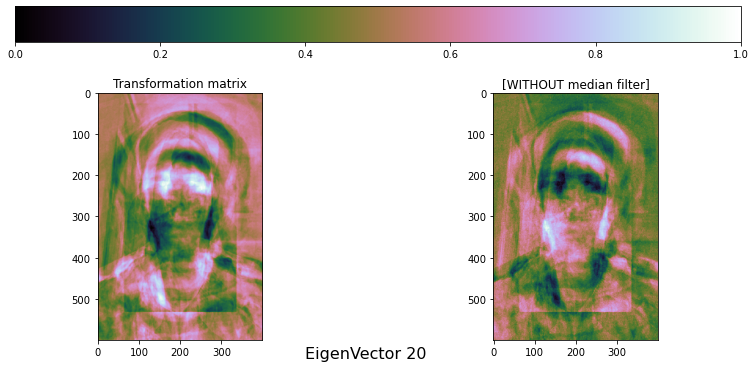
\includegraphics[width=.8\columnwidth]{eig_20.png}
    \caption{$d=20$时的特征向量输出}
    \label{fig:eig_20}
\end{figure}

颜色空间是按照百分比的方式(0~1)对归一化的特征向量进行绘制的。不同方式生成的特征向量,有时候会接近相似,有时会大相径庭,但有时候却会……完全相反?

\begin{figure}[H]
    \centering
    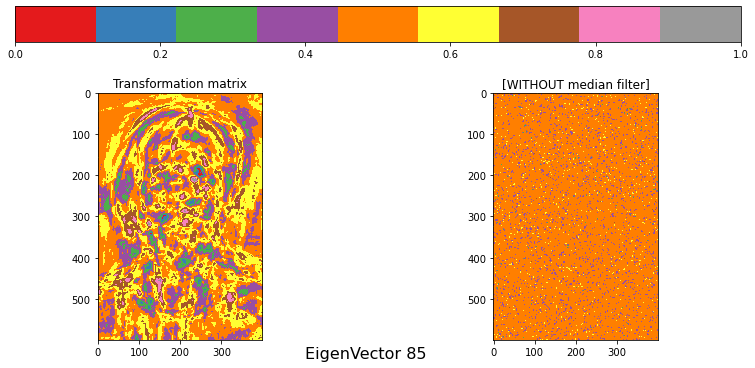
\includegraphics[width=.8\columnwidth]{eig1.png}
    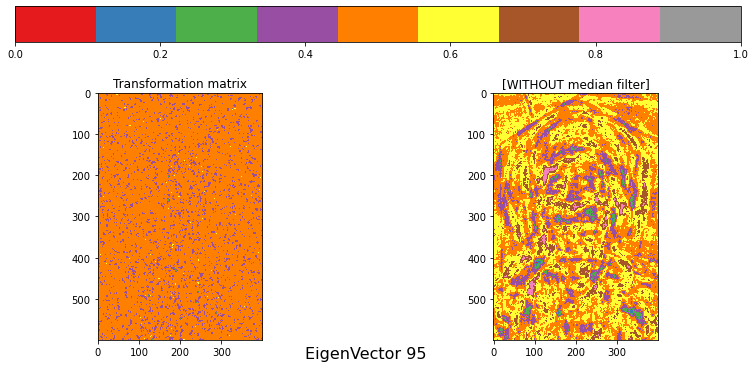
\includegraphics[width=.8\columnwidth]{eig2.png}
    \caption{$d=85$和$d=95$时的特征向量输出}
    \label{fig:eig}
\end{figure}

随着维数增大,两种特征向量里都出现了噪声形成的主成分,且中值滤波前的主成分为噪声的维数更多。这说明生成的噪声过于密集,造成了两个结果:

1.噪声重合形成了一定的规律,并被代数方法所单独识别出来。(这听上去就很无监督学习。)否则,噪声应基本在含有人脸的特征向量中显现。(实际上,两种特征向量里也都有这种情况)

2.套用的中值滤波方式仍不能很好的去除现有的噪声。

那么是时候总结一下了。
% \include{contents/analysis}
% \chapter{反思与总结}

总结本阶段实验,第一项实验给我留下了最深刻的印象。在我之前的认识中,图像的预处理在不同应用领域应当都有最常用的实现方式,甚至于可证明的最优解(State of art)。然后发现这里面的水还是太深了……要考虑的内容比神经网络相关的具体太多,而不是虚无缥缈地调参。同时,我甚至一直以为色彩转灰度只是简单的平均数计算,但对比的图像及其相应的结果都让人大吃一惊。这说明了人眼很容易被图像诓骗,但它又经常对变化敏感。那么,文献收下了,咱慢慢看。

在整理实验报告的时候才注意到滤波器还有很重要的一点没有考虑到,即其作用范围(滤波子的大小)。中值滤波选用稍大的滤波子时,可能会对该数据集的噪声有显著提升的抑制作用。但噪声最好也得用个工具,从信号的角度出发,量化测量一下,不然又得用肉眼看?这可不太好。

在本实验中,数据集有过拟合倾向,因此还应考虑选用其他人脸数据集进行测试,这样或许也能进一步验证我的猜想。不过本次实验也让我迷迷糊糊地认识了协方差矩阵这一个重要概念,老朋友以后见!

感谢老师、助教、同学和开源资料,以及所引参考文献的各作者。该实验的完成缺少不了你们的贡献。
\chapter{稀土元素发展和新材料应用初探}

随着科学技术的发展,人类的社会形态和生活方式在近几个世纪不断被革新。尤其是二十世纪以来,各类基础学科的重大发现和扩展应用加速了这一变化。具体到化学而言,十九世纪出现的水泥和钢筋混凝土,伴随着石油提炼方式的创造,带领着人类走入材料和能源的新纪元。二十世纪初投入工业制造和研究的无机金属和有机材料两大方向,则更是与前者相辅相成。\cite{gan2014da}

稀土元素也在此时发现并被投入到一些生产应用上。步入六十年代 ,伴随着稀土矿场的大规模开采和钐钴永磁体的发明,稀土元素开始了它的表演——它陆续被应用在电气原件生产和反应催化处理中,并在新世纪被赋能为新能源器械的灵魂元素。正因如此,在稀土元素的开采、加工、利用各阶段,我们要更好地运用绿色化学的思想,助力可持续发展,为碳中和贡献自己的力量。\cite{Atwood_2012,Balaram_2019,Institute_2020}

本文将基于上述背景,从化学和智能生活的角度出发,探究稀土元素在新材料中的应用。

\section{分类及开采}

\begin{figure}[H]
    \centering
    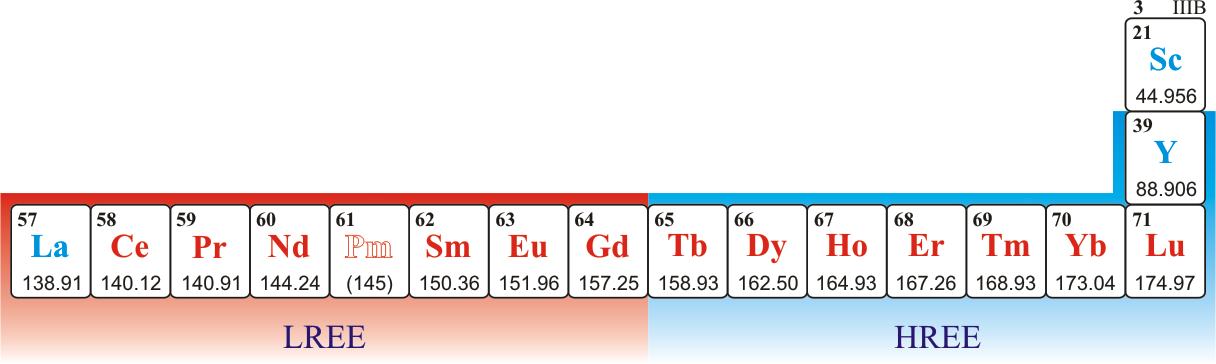
\includegraphics[width=0.9\columnwidth]{../images/ree_division.png}
    \caption{展示了稀土元素在元素周期表的位置和一种分类。\cite{Generalic_2012}\label{fg:division}}
\end{figure}
稀土元素(REE, Rare Earth Element),指的是元素周期表上第IIIB族的17种元素,包括钪(Scandium)、钇(Yttrium)和含镧(Lanthanum)在内的其他十五个镧系元素,并共享着类似的化学性质,例如:在简单化合物中,由于各元素原子的电子分布情况类似(\ce{4f^{0$\sim$14} 5d^{0$\sim$1} 6s^{2} }),最后增加的电子一般填充在f亚层中,它们均以正三价的形式存在。与之相对应的,粒子微小的变动导致它们之间有所区别,例如:钷(Promethium)是这些元素里的唯一一个放射性元素(严格来说也不算化学性质了)。另外,根据矿物分布及特征,和粒子半径及其导致的不同性质,稀土元素还被分为轻型重型两类,一种常见区分方法及其在元素周期表内的位置如\autoref{fg:division}。不同的分类方法\cite{Generalic_2012,Atwood_2012,baipi_2012}可能会从钐(Samarium)到镝(Dysprosium)选择某个元素作为重稀土(HREE, Hard Rare Earth Element)起始元素,而钪则一般不像钇一样归入重稀土元素,也不归入轻稀土(LREE, Light Rare Earth Element),而是单独成一类。

\begin{figure}[H]
    \centering
    \includesvg[width=0.6\columnwidth, pretex=\tiny]{../images/elemental-abundances.svg}
    \caption{展示了部分元素的各类型粒子在地球土壤中的丰度。\cite{Haxel_2002}\label{fg:abundances}}
\end{figure}

值得一提的是,稀土的名称正来源于“稀有的土壤成分”,但现代的地质学考证结果说明,它们的含量远比我们熟知的珍贵金属(Precious metals),如银、金等要高一个数量级。而铈(Cerium)作为地球土壤中丰度最高的稀土元素,更是得到了第27名的好成绩。可视化的数据可以看\autoref{fg:abundances},这张广泛引用的相对丰度图有力地展现了稀土元素的高含量。相比较而言,陨石中稀土元素含量往往还更少。\cite{Balaram_2019}

和老朋友铝很像,稀土元素的发现和制备的相关历史均较短,这和稀土元素活泼的性质是分不开的——他们在土壤矿质中均以化合物的形式存在,且各种元素混合在一起,需要合适的工艺进行分离,低效的工艺可能会将大量有效成分作为难以分离的杂质丢弃。\cite{Atwood_2012,张晔_2019}由于篇幅所限,此处不过多涉及开采和矿类加工的相关内容,这些信息在中文互联网上满地都是。(不会吧,不会真有人不知道中国的稀土勘探量和产量名列前茅吧)

\section{工业应用情况}

稀土早期曾应用于燃气灯覆盖层、抛光物质和玻璃上色等工艺中,而要系统地介绍当前稀土元素的各类用途和场景是很困难的。基于写一篇小论文的目标,此处不区分各元素地描述和日常场景相接近的三个用途:催化、磁性和超导,将简单介绍其相应的化学原理和实际应用产品。

稀土还用于荧光粉、玻璃添加剂、合金和有机材料合成等相关领域\cite{JohnHamiltonWalrod_2012a,Dawei_2018,DeakinUniversity_2012},但需要前置知识过多,而且内容杂碎,故这些应用虽然也很重要但此处不再涉及。

\subsection{用于催化过程}

稀土元素最早的工业应用,便是作为多相催化物(Heterogeneous Catalysis)用于冶金和石油化工工业。

在冶金工业中它们作为还原剂、脱氧剂和脱硫剂。在炼钢温度下反应\ce{2La + 3[O] <=>[1600 \textdegree{C}C] La2O3(s) }可很快发生平衡,例如钢中只要含$2\times10^{-4}\%$的镧,它的含氧质量分数便可降低至$1\times10^{-4}\%$。\cite{gan2014inbook}

同时,液化的稀土氧化物可取代传统的强酸强碱,在化工反应中替代沸石晶格中的某些重要成分,产生大量能量,并导致石油等物质催化裂化,甚至于酯的水解。值得注意的是,它们在600~800K以上的温度才有催化活性。\cite{JohnHamiltonWalrod_2012,金文_2015}
据记载,典型的催化氧化物有氧化铈(\ce{CeO2})、氧化镧(\ce{La2O3})和氧化钕(\ce{Nd2O3}),它们作为催化剂在2008年的年度消耗量就分别达到了6840 mt,380 mt和228 mt。\cite{Atwood_2012a}

作为多相催化物,稀土元素还有可能在汽车尾气处理、锅炉烟尘等方向继续发挥作用,促进尾气处理,实现环保的目标。如南京大学董林教授就在进行低温稀土铈基催化剂脱硝的研究和实践。\cite{张晔_2019}\footnote{\inlinecite{张晔_2019}这篇采访稿里其实有很多值得推敲的地方,比如\inlinecite{Atwood_2012a}就提到国际上销量最多的稀土元素应该是Ce, La, Nd, 全是轻稀土}此外,稀土作为均相催化剂(Homogeneous Catalysis)与有机物等物质相结合,也是目前研究的热点方向。\cite{Yao_2012a}

\subsection{用于磁性材料}

正如前述所言,稀土金属最早展现出了它在磁体方面的魅力,直到现在新材料、新科技的应用时代,这点仍显得尤为重要。就连加拿大某矿产公司主营市场经销的Pierre Neatby也坦言:“像钕磁铁,能做到重量轻而又有强磁力,所以用它来作电动汽车的引擎,就能更好地让它轻量化、小型化。正因如此,从\textbf{喷气飞机到军用潜艇再到新能源汽车},稀土元素都发挥着独特的作用。”\cite{Kirkpatrick_2019}就具体数据而言,一个3.5兆瓦功率的涡轮\textbf{风力发动机},便需要600千克的稀土永磁体材料。\cite{Atwood_2012a}

由于居里温度低,在室温下纯稀土物质并不显现磁性,但与过渡金属铁镍等形成化合物后,其磁性比铁氧体磁铁或陶瓷磁铁均要更强。它们的磁性来源于原子结构造成的高磁矩(4f轨道上未成对电子同向自旋),以及晶体结构的高磁向各异性。

传统来说,钕铁硼磁铁和钐钴磁铁(当然还含其他物质)这两种是最常见的永磁体。而未来对稀土磁体的研究,可能可以从不同的磁体排序材料,如链状磁、离子磁、原子磁等(SCM = single-chain magnets; SIM = single-ion
magnet; SMM = single-molecule magnets)\cite{Wang_2012a,Wang_2012}

\subsection{用于超导材料}

超导材料指的是在特定温度和压强下展现出零电阻的物质,且环境一般是低温高压(毕竟超导也是追求绝对零度的科研副产品)。所谓的\qthis{高温超导材料}(HTSC, high temperature superconductors)反而是指77K以上(液态氮气环境)可展现超导性质的物质,在这个条件下的超导将具有更为普遍的实用意义。

稀土元素很早就被用来进行高温超导研究,并在本世纪初利用稀土实现了120K以上的超导物质(见\autoref{fig:sc2012}),在去年更是有学者实现了室温高压的超导(居然不带稀土玩了,虽然你看发展轴上全是稀土,见\autoref{fig:sc2020})。

\begin{figure}[H]
	\begin{minipage}{0.45\textwidth}
		\centering
		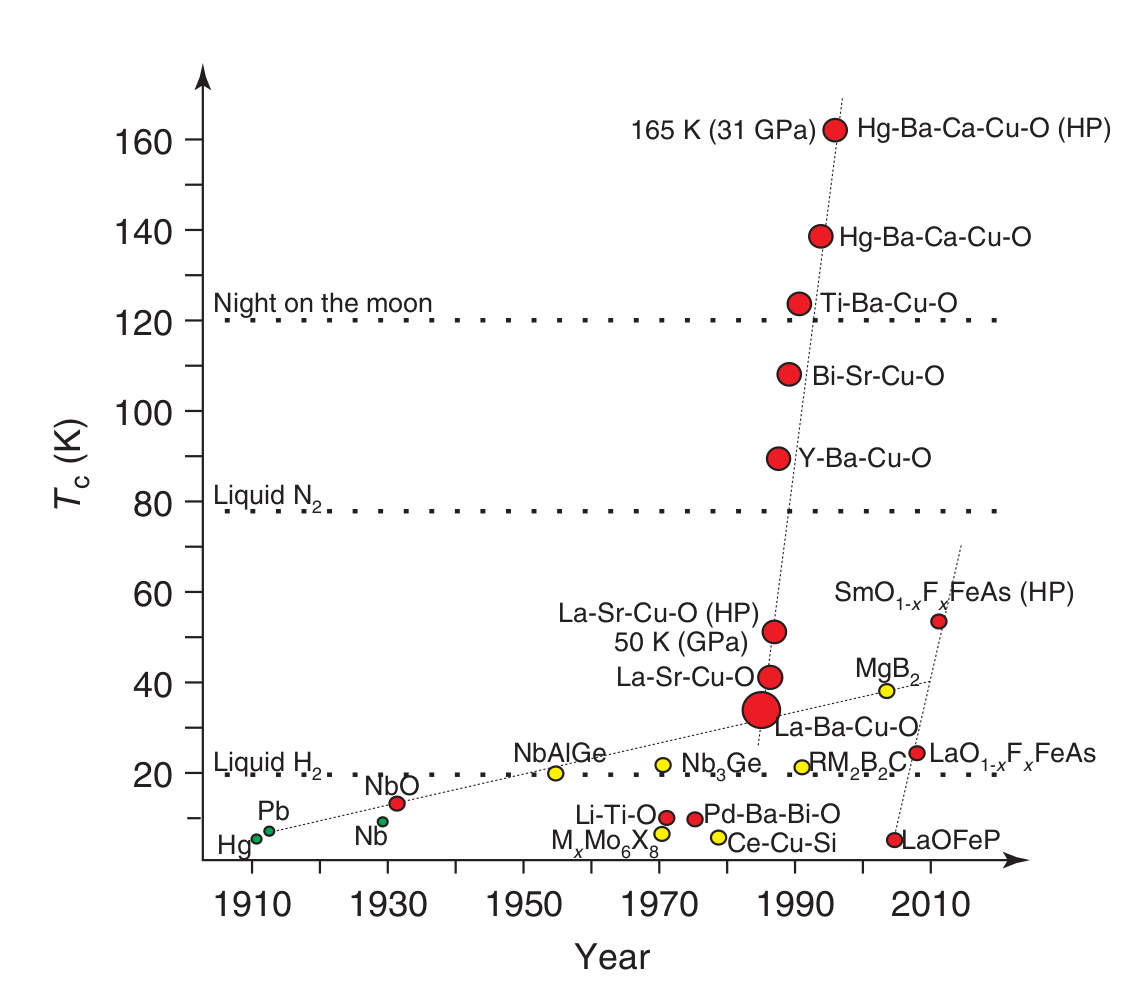
\includegraphics[width=1.05\columnwidth]{../images/superconduct1.png}
		\caption{\inlinecite{AntonioJ.DossantosGarcia_2012a}中展示的超导进化树}
		\label{fig:sc2012}
	\end{minipage}\hfill
	\begin{minipage}{0.45\textwidth}
		\centering
		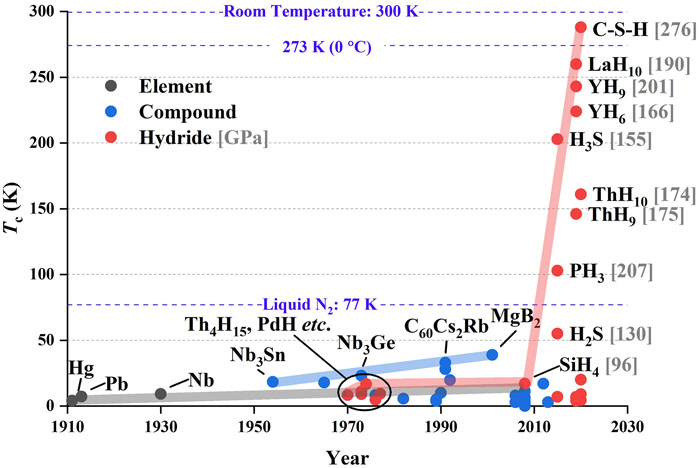
\includegraphics[width=1.05\columnwidth]{../images/superconduct2.jpg}
		\caption{\inlinecite{Lv_2020}中展示的超导进化树}
		\label{fig:sc2020}
	\end{minipage}
\end{figure}

距离我们生活最近的超导材料便是磁悬浮(它和强磁性无关),它应用了迈斯纳效应(Meissner effect),西南交通大学的超高速真空管道磁悬浮交通研究中心正力图从传统的电磁悬浮、电动悬浮两种磁悬浮方式中吸收经验,利用研究成果应用于高温超导悬浮。2021年1月,设计时速620公里的样车和设计线已与媒体见面,其技术和制造工艺均为国产原创,它是西南交通大学联合中车公司、中国中铁等单位协同攻关研发的项目,旨在让技术走出实验室,迈出验证其高速运行可靠性的第一步。高温超导甚至还可以用于普通马达的储能,这也将是一个前沿应用方向\cite{AntonioJ.DossantosGarcia_2012a,王迪_2021}

题外话:如果用超导微观的BCS理论(Bardeen–Cooper–Schrieffer theory)来研究这个现象,那么这些稀土元素的磁性和超导特性的原理都是一样的。另外如果只涉及到导体,钕和钐的氧化物还是陶瓷电容(C0G (NP0))的主要成分,这种电容具有温度补偿特性,是电容量及介质损耗最稳定的电容器之一。具体来说,集成电路上广泛用到这种电容。\cite{Kaye_2020}

\section{结语}

本文通过简述传统化工材料的路径,并描绘稀土元素和新材料的发展,展现了当下化学知识及其应用与智能生活密不可分的关系,运用这些知识有助于我们构造环境友好型社会。同时,\inlinecite{Atwood_2012}这本书对稀土的基本化学性质、有代表性的化合物、以及一些常见形态和应用方式进行了说明,对我撰写上述内容时起到了很大的帮助(同时有些专业知识也让我陷进去了)。根据系列序言,该书是EIBC(Encyclopedia of Inorganic and Bioinorganic Chemistry)的一部分,并旨在为初学者和研究者提供翔实的参考资料。

需要注意本文引用的数据仅供说明使用,不构成任何对比或事实阐述,含数字的内容均有文献参考,但其准确性仅供参考。市场分析自己去看,不构成投资建议。\cite{baipi_2012,Fernandez_2017}(说白了,定性说话不腰疼,定量说话要挨打)

参考文献等原始数据,参见\url{https://github.com/tiger3018/hw/blob/HEAD/chemistry}。


\backmatter %%% 后置部分(致谢、参考文献、附录等)


%% 致谢
% \include{contents/ack}
%% 参考文献
% 顺序编码制:cqunumerical		
% 注意:至少需要引用一篇参考文献,否则下面两行会引起编译错误。
\bibliographystyle{cqunumerical}
\bibliography{ree}

\end{document}